% Supplied Project-2026 template; build_paper.ps1 runs Tectonic.
% The original template is unchanged. Font, class, columns and margins match it.
% Group and equal author contributions supplied by the students.
% Numeric tables and the matrix are generated from one experiment in paper_assets/.
\documentclass[twocolumn,10pt]{article}

\usepackage{authblk}
\usepackage{bera}
\usepackage[utf8]{inputenc}
\usepackage[T1]{fontenc}
\usepackage{booktabs}
\usepackage{graphicx}
\usepackage[numbers,sort&compress]{natbib}
\usepackage{url}
\usepackage[hidelinks]{hyperref}

\title{Cross-Label Duplicates in Clinical Text}
\author{\normalsize Group 64 --- Tiago Pinto (25\%), Gonçalo Narciso Rolo (25\%)\\
\normalsize Gabriel Alexandre Lino Simões Ferreira (25\%), Miguel Neves Antão Ermida Parreira (25\%)}
\date{}

% Measured summaries are edited manually; tables are rebuilt from recorded CSVs.
\newcommand{\AugmentationOutcome}{LR mixtures lower R+EX macro F1
from 73.27\% to 70.13\%. SVC mixtures pass, but copies match rounded R+EX
macro/Dermatology F1 (75.45/54.17\%).
Promotion does not establish a lexical benefit.}
\newcommand{\MainResultSummary}{For selected SVC+mix, EX raises R accuracy
from 47.28\% to 77.41\%. All 1,269 matched validation labels are absent
from training matches. Versus unaugmented SVC+EX, Dermatology
precision rises 44.8\% to 56.5\%, with recall unchanged at 52\% (13/25).}
\newcommand{\ErrorDiscussion}{Case 1892, \emph{Wrist Ganglion Excision}: supplied Surgery, predicted Orthopedic.
``After administering appropriate antibiotics and general anesthesia, the upper
extremity was prepped and draped in the usual standard fashion. The arm was
exsanguinated with an Esmarch and tourniquet inflated to 250 mmHg. I made a
transverse incision directly over the ganglion.'' Operative language and wrist
anatomy plausibly suggest different tags; EX has no training match.
This is interpretation, not feature attribution.\par
Case 309, \emph{Cheek-Neck Facelift}: supplied Dermatology, predicted Radiology.
``Temporal cheek-neck facelift (CPT 15825). Submental suction assisted lipectomy
(CPT 15876)\ldots{} This patient is a 65-year-old female who has progressive aging
changes of the face and neck. The patient demonstrates the deformities described
above and has requested surgical correction.''
EX masks Surgery from an identical training copy but chooses an incorrect
remaining label.\par
Case 1383, \emph{Anterior Lumbar Fusion}: supplied Orthopedic, predicted Neurosurgery.
``Dr. X made the approach and once we were at the L5-S1 disk space, we removed
the disk and we placed a 13-mm PEEK vertebral spacer filled with a core of bone
taken from the L5 vertebral body.'' Identical corpus copies carry Orthopedic,
Neurosurgery and Surgery. Only Surgery is masked here; Neurosurgery remains
available, illustrating ambiguity in these corpus annotations.\par}
\newcounter{bodypages}
\newcounter{documentpagecount}

\begin{document}
\maketitle

\section{Introduction}
Clinical notes can carry competing specialty labels. We ask:
\emph{How does cross-label duplication affect the evaluation and prediction of
medical specialties from clinical text?} Collection-dependent rules can limit
transfer~\citep{geirhos2020shortcut}.

\section{Data}
\subsection{Data Analysis}
CSV repairs retain 2,669 cases, 12 specialties and supplied labels. Surgery
contributes 893 cases (33.5\%), versus Dermatology's 25 (0.9\%). Cross-label
copies affect 1,528 cases (57.2\%), including 72/79 Neurosurgery cases;
descriptions, titles and transcriptions are identical. Incomplete records remain. We exclude
\texttt{keywords}: all 2,219 nonempty values start with the target specialty.

\subsection{Data Augmentation}
To diversify minority-class n-grams, we recombine sections~\citep{yoon2021ssmix}.
For the four classes with $n<100$ (Table~\ref{tab:classes}), each eligible training
note yields one variant borrowing a complete same-heading body from a same-class
original in another duplicate group. Both notes need two distinct headings and
chosen bodies of at least eight words. Titles/other sections remain unchanged;
SHA-256(seed~0, fold, record ID) selects pairs. Five Dermatology examples were
inspected before fitting: note 300's ``A 14-day-old...'' history receives 308's
``This 34-year-old gentleman...''; infant sections remain, demonstrating clinical
inconsistency. Copies repeat the same sources. Five-fold totals are 641 R/645 G
mixtures, reused by LR/SVC.

\section{Models}
Using scikit-learn~\citep{pedregosa2011scikit}, multinomial Naive Bayes (NB)
follows the reference: lowercased, Porter-stemmed \texttt{description} TF-IDF,
Laplace smoothing ($\alpha=1$) and empirical priors.
Logistic regression (LR) and linear support vector classification (SVC) provide
n-gram baselines~\citep{wang2012baselines}. They use separately L2-normalised
\texttt{sample\_name}/\allowbreak\texttt{transcription} TF-IDF blocks.
Both compare originals, mixtures and copies; NB also differs in representation.

Exclusion (EX) masks labels from original training-fold matches of the lowercased,
whitespace-normalised title/transcription pair, choosing the highest remaining
score. Empty/no-match/all-masked cases use raw prediction; NB uses the same lookup.
Unseen-label continuation is a corpus hypothesis, not a clinical rule.

\begin{table}[!t]
\centering
\small
\setlength{\tabcolsep}{3pt}
\begin{tabular}{@{}llrrr@{}}
\toprule
System & CV & Acc. & Macro F1 & Min. F1 \\
\midrule
NB & R & 38.67 & 13.23 & 0.00 \\
NB & R+EX & 55.41 & 35.35 & 0.00 \\
NB & G & 41.14 & 15.26 & 0.00 \\
LR (B) & R & 48.78 & 51.81 & 31.86 \\
LR (B) & R+EX & 76.62 & 73.27 & 47.76 \\
LR (B) & G & 55.75 & 58.19 & 45.08 \\
SVC & R & 46.16 & 49.77 & 23.82 \\
\textbf{SVC} & \textbf{R+EX} & \textbf{77.56} & \textbf{75.26} & \textbf{48.15} \\
SVC & G & 57.10 & 60.28 & 43.51 \\
\bottomrule
\end{tabular}

\caption{Out-of-fold results (\%). R: rows; G: grouped notes; EX: exclusion.
Bold: selected. Grouped EX equals raw.}
\label{tab:systems}
\end{table}

\begin{table}[!t]
\centering
\small
\setlength{\tabcolsep}{3pt}
\begin{tabular}{@{}lrrrrr@{}}
\toprule
Specialty & $n$ & $P_R$ & $R_R$ & $F1_R$ & $F1_G$ \\
\midrule
1 Cardiovasc.-Pulm. & 309 & 76.4 & 82.8 & 79.5 & 61.8 \\
2 Dermatology & 25 & 44.8 & 52.0 & 48.1 & 50.0 \\
3 Gastroenterology & 195 & 72.4 & 79.5 & 75.8 & 60.0 \\
4 General Medicine & 212 & 69.6 & 86.3 & 77.1 & 77.4 \\
5 Neurology & 184 & 69.2 & 73.4 & 71.2 & 58.0 \\
6 Neurosurgery & 79 & 55.5 & 83.5 & 66.7 & 45.0 \\
7 Obstetrics-Gynecol. & 136 & 72.6 & 87.5 & 79.3 & 63.3 \\
8 Ophthalmology & 73 & 77.8 & 95.9 & 85.9 & 72.3 \\
9 Orthopedic & 300 & 73.5 & 84.0 & 78.4 & 58.2 \\
10 Psychiatry-Psychol. & 41 & 85.7 & 87.8 & 86.7 & 82.8 \\
11 Radiology & 222 & 74.0 & 74.3 & 74.2 & 51.1 \\
12 Surgery & 893 & 95.1 & 69.4 & 80.3 & 43.5 \\
\bottomrule
\end{tabular}

\caption{Selected-system support, row-wise precision/recall/F1 and grouped F1 (\%).}
\label{tab:classes}
\end{table}

\begin{figure}[!t]
\centering
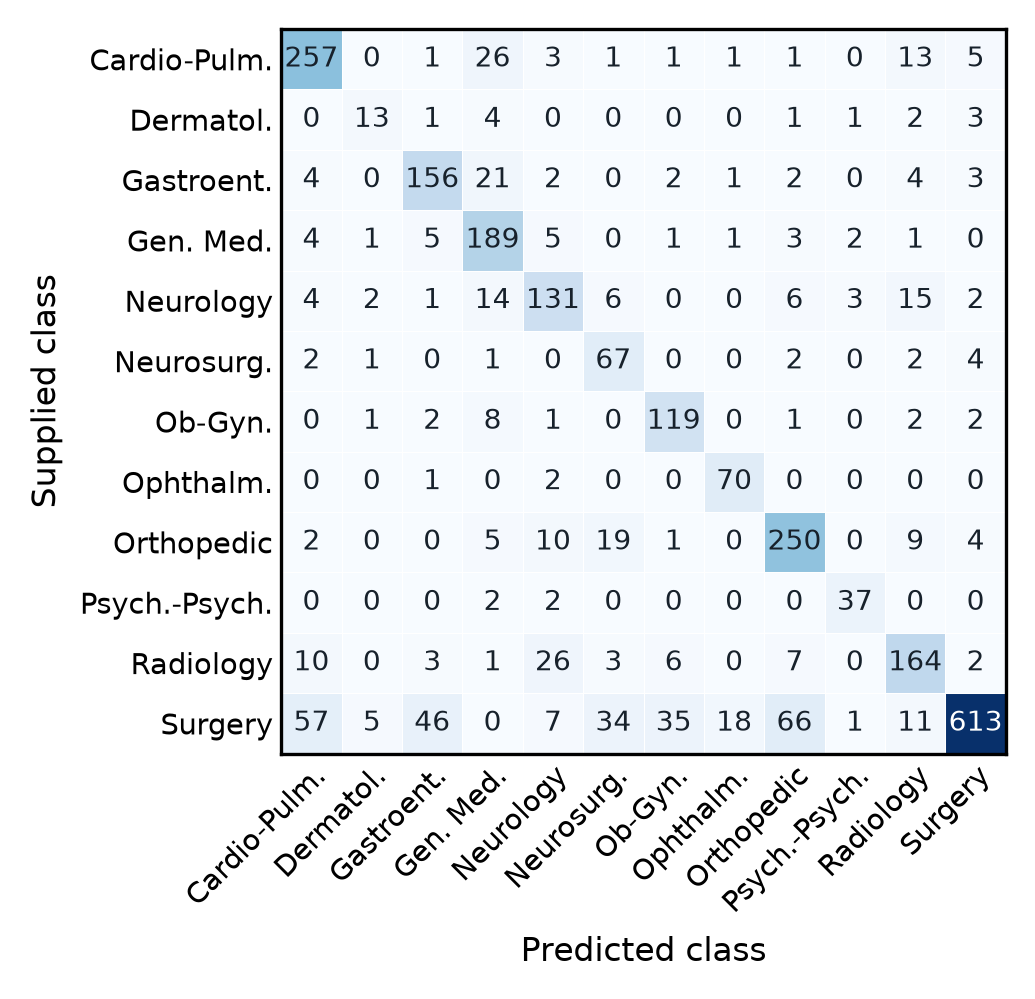
\includegraphics[width=\columnwidth]{paper_assets/confusion_matrix.png}
\caption{Selected-system row-wise confusion matrix. Rows: supplied labels;
columns: predictions. Class order: Table~\ref{tab:classes}.}
\label{fig:confusion}
\end{figure}

\section{Experimental Setup}
Five-fold \texttt{StratifiedKFold} over rows (R) and
\texttt{StratifiedGroupKFold} over notes (G) are shuffled with seed~0;
seven configurations with/without EX share folds within each protocol.
G groups normalised transcriptions, using titles when absent and unique IDs
when both fields are empty. Features, weights, augmentation and EX indices use training folds
only; pooled validation originals yield accuracy, macro F1 and per-class metrics.
EX is inactive in G, which tests unseen notes within this corpus.
Choices remain exploratory~\citep{cawley2010overfitting}.
Before recombination fits, promotion required R+EX macro/Dermatology F1
improvements over family originals and SVC+EX, at most one accuracy point loss,
accuracy $>49\%$ and all-class F1 $\geq25\%$. Passing mixtures rank by macro F1,
Dermatology F1, then accuracy; otherwise SVC+EX remains. The official 398-case
test only generates predictions; its scores are unavailable.

\subsection{Parameters/Hyperparameters}
LR/SVC use lowercased word unigram/bigram TF-IDF, sublinear term frequency,
\texttt{min\_df=2} (minimum document frequency), no stemming/stopword removal,
L2, $C=0.25$ (inverse
regularisation) and at most 2,000 iterations. LR uses multinomial log loss;
SVC uses one-versus-rest squared hinge.
TF-IDF refits on originals and additions. LR/SVC weights $N/(12n_c)$ use
original sample/class counts; after assignment to originals/additions, total
weight is normalised to $N$. Copies control increased source influence;
mixing also changes TF-IDF.

\section{Results}
Tables~\ref{tab:systems}--\ref{tab:classes} give overall/per-class results;
Figure~\ref{fig:confusion} shows R confusions.
\MainResultSummary{} \AugmentationOutcome{}

\section{Discussion}
Surgery to Orthopedic is the most frequent remaining confusion (66 cases).
\ErrorDiscussion{}
Cross-label copies create conflicting supervision yet enable annotation
completion, answering the research question. EX's corpus assumption can fail
on repeated labels; approximate copies, patient dependence and selection bias
remain. Synthetic patient coherence is distinct from predictive benefit.

\section{Future Work}
Independent collections, adjudicated multi-label notes and clinician-reviewed
augmentation would test transfer; nested selection would limit development bias.

\paragraph{LLM use.}
ChatGPT assisted data preprocessing and LaTeX preparation;
Claude helped check theoretical reasoning.

% The user's stricter limit includes references: no forced bibliography page.
\setcounter{bodypages}{\value{page}}
\typeout{PAPER BODY PAGES=\arabic{bodypages}}
\renewcommand{\refname}{Bibliography}
\begingroup
\small
\setlength{\bibsep}{2pt}
% Compact references; complete bibliographic metadata remains in paper.bib.
\begin{thebibliography}{5}
\bibitem{geirhos2020shortcut}
R. Geirhos et al.
\href{https://doi.org/10.1038/s42256-020-00257-z}{Shortcut Learning in Deep Neural Networks}.
\emph{Nature Machine Intelligence}, 2020.

\bibitem{yoon2021ssmix}
S. Yoon, G. Kim and K. Park.
\href{https://aclanthology.org/2021.findings-acl.285/}{SSMix: Saliency-Based Span Mixup for Text Classification}.
\emph{Findings of ACL-IJCNLP}, 3225--3234, 2021.

\bibitem{pedregosa2011scikit}
F. Pedregosa et al.
\href{https://jmlr.org/papers/v12/pedregosa11a.html}{Scikit-learn: Machine Learning in Python}.
\emph{JMLR}, 12:2825--2830, 2011.

\bibitem{wang2012baselines}
S. Wang and C. Manning.
\href{https://aclanthology.org/P12-2018/}{Baselines and Bigrams: Simple, Good Sentiment and Topic Classification}.
\emph{ACL}, 90--94, 2012.

\bibitem{cawley2010overfitting}
G. C. Cawley and N. L. C. Talbot.
\href{https://jmlr.org/papers/v11/cawley10a.html}{On Over-fitting in Model Selection and Subsequent Selection Bias in Performance Evaluation}.
\emph{JMLR}, 11:2079--2107, 2010.
\end{thebibliography}

\endgroup

\clearpage
\setcounter{documentpagecount}{\value{page}}
\addtocounter{documentpagecount}{-1}
\typeout{PAPER TOTAL PAGES=\arabic{documentpagecount}}
\ifnum\value{documentpagecount}>3
  \PackageWarningNoLine{paper}{Entire PDF exceeds three pages, including references}
\fi
\end{document}
